\chapter{Proximal mappings}
\label{chap:proximal_mappings}

In this chapter we cover a useful concept that generalizes the notion of
(Euclidean) projection onto a given set to an operator which ``proximity'' to
its input, guided by a given function.

\section{Definition and properties}

The \emph{proximal mapping} (also called proximal map, or proximal operator)
associated with a function $f : \R^d \to [-\infty, \infty]$ is a set-valued map,
denoted by $\prox_f$, that maps each $x \in \R^d$ to a subset of $\R^d$
(possibly the empty set), defined by           
\index{proximal mapping}
\begin{equation}
\label{eq:proximal_mapping}
\prox_f(x) = \argmin_z \bigg\{ \frac{1}{2} \|x - z\|_2^2 + f(z) \bigg\}. 
\end{equation}
Here and throughout, we denote by $\argmin_{z \in S} F(z)$ the set of
minimizers of a function $F$ over a set $S$, and denote by $\argmin_z F(z)$ 
the set of minimizers of $F$ over its entire effective domain. We will abide by
the common convention that $\argmin$ returns the minimizer itself when the
latter is unique (not the set containing the minimizer).     

As mentioned, we can think of $\prox_f$ as a generalization of the projecton map
onto a set. Indeed for $f = I_C$, the characteristic function of a set $C$,  
\index{projection}
\begin{equation}
\label{eq:proximal_mapping_projection}
\prox_f(x) = P_C(x) = \argmin_{z \in C} \, \|x - z\|_2.
\end{equation}
Keeping this connection in mind will generally be helpful for developing
intuition about proximal maps because---as we will see in what follows---the  
proximal map associated with a closed convex function shares several useful
properties of projection onto a closed convex set. 

A slight variation on \eqref{eq:proximal_mapping} will be of central interest in
this chapter,  
\index{proximal mapping}
\begin{equation}
\label{eq:proximal_mapping_lambda}
\prox_{\lambda f}(x) = \argmin_z \bigg\{ \frac{1}{2\lambda} \|x - z\|_2^2 + 
f(z) \bigg\},  
\end{equation}
which is simply the proximal map associated with the scaled function $\lambda f$
for $\lambda > 0$. An intimately related object looks at the infimum (rather
than the minimizer), 
\index{Moreau envelope}
\begin{equation}
\label{eq:moreau_envelope_lambda}
f_\lambda(x) = \inf_z \bigg\{ \frac{1}{2\lambda} \|x - z\|_2^2 + f(z)
\bigg\}, 
\end{equation}
called the \emph{Moreau envelope} of $\lambda f$, which will be studied a bit
later in Chapter \ref{sec:moreau_envelope}. 

We now discuss some basic properties and interpretations of proximal
mappings. We generally assume henceforth that $f \not= \infty$ ($\dom(f) \not= 
\emptyset$) to rule out trivialities when studying proximal maps.      

\paragraph{Existence and uniqueness.}

First we discuss a case where the proximal mapping acts as a well-defined 
function, from $\R^d$ to $\R^d$. If $f$ is closed and convex, then for any
$\lambda > 0$ the function    
\[
z \mapsto \frac{1}{2\lambda} \|x - z\|_2^2 + f(z)
\]
is closed and strongly convex. For the proximal mapping
\eqref{eq:proximal_mapping_lambda} to be a function (single-valued rather than
set-valued), we need a minimizer of the function in the above display to exist
and be unique. Existence comes from Weirstrass' theorem (Theorem
\ref{thm:weierstrass}), along with the fact that strongly convex functions are
coercive (Exercise \ref{ex:strong_convexity_coercive}). Uniqueness comes from
the fact that strictly (thus strongly) convex functions have at most one
minimizer (Exercise \ref{ex:convex_solution} part d). We summarize this next. 

\index{proximal mapping!existence and uniqueness}
\begin{Theorem}
\label{thm:proximal_existence_uniqueness}
For a closed and convex function $f : \R^d \to (-\infty, \infty]$ with nonempty
domain, and for any $\lambda > 0$, the proximal map
\eqref{eq:proximal_mapping_lambda} is a well-defined function: it maps each
point in $x \in \R^d$ to a point $\prox_{\lambda f}(x) \in \R^d$.   
\end{Theorem}
\vspace{-3pt}

\paragraph{Subgradient characterization.}

For closed convex $f$, the optimization problem 
\[
\minimize_z \quad \frac{1}{2\lambda} \|x - z\|_2^2 + f(z)
\]
has a subgradient optimality condition: $0 \in (z - x) / \lambda + \partial
f(z)$, that is, $x - z \in \lambda \partial f(z)$. (Convexity is used here to
write the subdifferential of a sum as a sum of subdifferentials, by Property 
\parref{par:subgradient_sum}.) Therefore by subgradient optimality, we get $z =
\prox_{\lambda f}(x)$ if and only if 
\index{proximal mapping!subgradient characterization}
\begin{equation}
\label{eq:proximal_subgradient_characterization}
x - z \in \lambda \partial f(z),
\end{equation}
which we call the subgradient characterization of the proximal operator
associated with $\lambda f$. 

For $f = I_C$, the characteristic function of a convex set $C$, if we set (say)
$\lambda = 1$, and recall that $\partial I_C(z) = N_C(z)$, the normal cone to
$C$ at $z$, then we can see that
\eqref{eq:proximal_subgradient_characterization} reduces to the variational
inequality \eqref{eq:variational_inequality} for the projection $z = P_C(x)$ of
$x$ onto $C$.

\paragraph{Gradient step interpretation.}

The subgradient characterization
\eqref{eq:proximal_subgradient_characterization} leads to a nice interpretation
for \smash{$\prox_{\lambda f}(x)$} when $f$ convex and differentiable. In this
case, note that \eqref{eq:proximal_subgradient_characterization} becomes a
fixed-point equation for \smash{$z = \prox_{\lambda f}(x)$},  
\begin{equation}
\label{eq:proximal_fixed_point}
z = x - \lambda \nabla f(z).
\end{equation}
For small $\lambda$, it is reasonable to assume that \smash{$z = \prox_{\lambda
    f}(x)$} will be close to $x$ (as the term $\|x - z\|_2^2$ in the criterion
in \eqref{eq:proximal_mapping_lambda} will be multiplied by a large weight), so 
replacing $\nabla f(z)$ with $\nabla f(x)$ in the fixed-point equation
\eqref{eq:proximal_fixed_point} gives the approximation  
\begin{equation}
\label{eq:proximal_gradient_step_approx}
\prox_{\lambda f}(x) \approx x - \lambda \nabla f(x).
\end{equation}
That is, for small $\lambda$, we can interpret \smash{$\prox_{\lambda f}(x)$} as 
performing a gradient descent step starting at $x$, with step size $\lambda$. We 
will return to this interpretation in Chapter \ref{sec:moreau_envelope}, when we
will be able to make a more precise statement involving the Moreau envelope.    

\paragraph{Resolvent of subdifferential.}

A transformation of the subgradient characterization
\eqref{eq:proximal_subgradient_characterization} yields another important  
interpretation for the proximal operator. Rearranging the right-hand side in
\eqref{eq:proximal_subgradient_characterization}, and using $I$ for the identity
map, we get
\begin{align*}
z = \prox_{\lambda f}(x) &\iff x \in (I + \lambda \partial f)(z) \\
&\iff z \in (I + \lambda \partial f)^{-1}(x).
\end{align*}
Here, we should interpret $I + \lambda \partial f$ as a set-valued map: in
general, it evaluates to $(I + \lambda \partial f)(z) = \{ z + \lambda s : s \in
\partial f(z) \}$, and its preimage to $(I + \lambda \partial f)^{-1}(x) = \{ z
: x \in (I + \lambda \partial f)(z) \}$. Inspecting the last display carefully,
we can see that it reveals something interesting: the preimage appearing in the
above line must actually be \emph{single-valued}, because there is exactly one 
point \smash{$z = \prox_{\lambda f}(x)$} which satisfies $z \in (I + \lambda
\partial f)^{-1}(x)$. This allows us to write 
\index{proximal mapping!resolvent of subdifferential}   
\begin{equation}
\label{eq:proximal_resolvent_characterization}
\prox_{\lambda f} = (I + \lambda \partial f)^{-1},
\end{equation}
where we interpret both the left- and right-hand sides in
\eqref{eq:proximal_resolvent_characterization} as single-valued mappings. This
is a representation for the proximal map in terms of what is called the 
\emph{resolvent} of the subdifferential.  

\medskip

\begin{Example}
\label{xa:proximal_mappings}
The following are examples of proximal maps of general interest in statistics
and machine learning. In each case, the stated result can be derived using the 
subgradient characterization \eqref{eq:proximal_subgradient_characterization} 
for the proximal operator.

\begin{enumerate}[label=\alph*., ref=\alph*]
\item For $f(x) = \frac{1}{2} x^\T A x + b^\T x + c$ with $A \succeq 0$, we have 
  \[
  \prox_{\lambda f}(x) = (I + \lambda A)^{-1} (x - \lambda b).
  \]

\item \parlab{xa:l1_norm_proximal_mapping} 
  For $f(x) = \|x\|_1$, we have (Exercise \ref{ex:lp_norm_proximal_mapping} part 
  a): 
  \index{l1 norm@$\ell_1$ norm!proximal mapping}
  \[
  [\prox_{\lambda f}(x)]_i = [s_\lambda(x)]_i 
  = \sign(x_i) \cdot (|x_i| - \lambda)_+, \quad i = 1,\dots,d.  
  \]
  where recall $a_+ = \max\{a, 0\}$ gives the positive part of $a$, and we
  interpret $\sign(0) = 1$. The operator $s_\lambda$ is called (coordinatewise)
  \emph{soft-thresholding} at the level $\lambda$, equivalently   
  \index{soft-thresholding}
  \begin{equation}
  \label{eq:soft_thresholding}
  [s_\lambda(x)]_i = 
  \begin{cases}
  x_i - \lambda & \text{if $x_i > \lambda$} \\
  0 & \text{if $|x_i| \leq \lambda$} \\
  x_i + \lambda & \text{if $x_i < -\lambda$}
  \end{cases},
  \quad i = 1,\dots,d.
  \end{equation}

\item \parlab{xa:l2_norm_proximal_mapping}  
  For $f(x) = \|x\|_2$, we have (Exercise \ref{ex:lp_norm_proximal_mapping} part
  b): 
  \[
  \prox_{\lambda f}(x) = \bigg(1 - \frac{\lambda}{\|x\|_2} \bigg)_+ x.
  \]

\item \parlab{xa:trace_norm_proximal_mapping} 
  For $f(X) = \|X\|_{\tr}$, the trace norm, and $X = U \Sigma V^\T$ denoting the
  SVD of $X$, we have (Exercise \ref{ex:matrix_norm_proximal_mapping1} part a):      
  \index{trace norm!proximal mapping}
  \[
  \prox_{\lambda f}(X) = U \diag(s_\lambda(\sigma)) V^\T.
  \]
  where $\sigma$ is the vector of singular values (the diagonal of $\Sigma$),
  $s_\lambda$ is the soft-thresholding operator defined above, and we use $A =
  \diag(a)$ to construct a diagonal matrix $A$ from a vector of diagonal
  elements $a$. The proximal operator here is typically denoted $m_\lambda$, and
  called \emph{matrix soft-thresholding}.
  \index{matrix soft-thresholding}

\item \parlab{xa:frobenius_norm_proximal_mapping}  
  For $f(X) = \|X\|_F$, the Frobenius norm, we have (Exercise
  \ref{ex:matrix_norm_proximal_mapping1} part b):    
  \index{Frobenius norm!proximal mapping}
  \[
  \prox_{\lambda f}(X) = \bigg(I - \frac{\lambda}{\|X\|_F} \bigg)_+ X,
  \] 
  where $A_+$ returns the elementwise positive part of a matrix $A$. 

\item \parlab{xa:l0_norm_proximal_mapping}   
  For $f(x) = \|x\|_0$, the $\ell_0$ norm (recall this returns the number of
  nonzero values, as in \eqref{eq:l0_norm}; it is nonconvex and \emph{not}  
  actually a norm) we have (Exercise \ref{ex:lp_norm_proximal_mapping} part c):   
  \index{l0 norm@$\ell_0$ norm!proximal mapping}
  \index{hard-thresholding}
  \[
  [\prox_{\lambda f}(x)]_i = [h_\lambda(x)]_i 
  = x_i \cdot 1\{|x_i| > \lambda\}, \quad i = 1,\dots,d.
  \]  
  The operator $h_\lambda$ is known as (coordinatewise) \emph{hard-thresholding}
  at the level $\lambda$. 

\item \parlab{xa:rank_proximal_mapping}    
  For $f(x) = \rank(X)$ (recall this is nonconvex), and $X = U \Sigma V^\T$
  denoting the SVD of $X$, we have (Exercise
  \ref{ex:matrix_norm_proximal_mapping2} part c):  
  \[
  \prox_{\lambda f}(X) = U \diag(h_\lambda(\sigma)) V^\T,
  \]
  where $h_\lambda$ is the hard-thresholding operator as defined above.
\end{enumerate}
\end{Example}

What can we do when the proximal operator is not available in closed-form? In
some settings, fast computaton may still be possible using specialized
techniques.  

\begin{Example}
\label{xa:proximal_mappings_efficient}
The examples below highlight interesting proximal mappings that cannot be 
computed in closed-form, but can still be efficiently evaluated using
specialized  algorithms.     

\begin{enumerate}[label=\alph*., ref=\alph*]
\item Let $y_i \in \R$, $i = 1,\dots,n$ be independent draws from an
  exponential family distribution with distinct natural parameters $\eta_i \in
  \R$, $i=1,\dots,n$, but a common sufficient statistic $T : \R \to \R$ and
  log-partition function $\psi : \R \to \R$. The negative log likelihood 
  is       
  \[
  f(\eta) = \sum_{i=1}^n \Big( \psi(\eta_i) - T(y_i) \eta_i \Big),
  \]
  where we have dropped terms not depending on $\eta$. The associated proximal
  operator 
  \index{exponential family!proximal mapping}
  \[
  \prox_{\lambda f}(\eta) = \argmin_{u} \bigg\{ \frac{1}{2} \|\eta - u\|_2^2 +
  \lambda \sum_{i=1}^n \Big( \psi(u_i) - T(y_i) u_i \Big) \bigg\}
  \]
  is not generally available in closed-form, but is efficiently computable for
  differentiable convex $\psi$ (recall that $\psi$ is always convex in any
  exponential family distribution). First note that the proximal map decomposes
  across coordinates: for each $i=1,\dots,n$,    
  \[
  [\prox_{\lambda f}(\eta)]_i = \argmin_{u_i} \bigg\{ \frac{1}{2} (\eta_i -
  u_i)^2 + \lambda \Big( \psi(u_i) - T(y_i) u_i \Big) \bigg\}. 
  \]
  The first-order optimality condition for the above problem is 
  \[
  u_i + \lambda \psi'(u_i) = \eta_i + \lambda T(y_i),
  \]
  a nonlinear equation in univariate $u_i$. The left-hand side is monotone
  nondecreasing in $u_i$, so the solution can be iteratively approximated with
  (say) binary search.       

\item \parlab{par:tv_proximal_mapping}
  The \emph{total variation (TV) penalty} is defined as
  \index{total variation (TV) penalty}
  \begin{equation}
  \label{eq:tv}
  f(x) = \sum_{i=1}^{d-1} |x_{i+1} - x_i|.
  \end{equation}
  This is a convex function (it is a seminorm). Its proximal operator    
  \index{total variation (TV) penalty!proximal mapping}
  \[
  \prox_{\lambda f}(x) = \argmin_z \bigg\{ \frac{1}{2} \|x - z\|_2^2 + 
  \lambda \sum_{i=1}^{d-1} |z_{i+1} - z_i| \bigg\}
  \]
  is efficiently computable (in linear-time, by which we mean the number of
  operations grows linearly in the dimension $d$) with dynamic programming or  
  taut string methods.       

\item \parlab{par:slope_proximal_mapping}
  The \emph{sorted $\ell_1$ penalty (SLOPE)} is defined, for constants
  $\lambda_1 \geq \cdots \geq \lambda_d \geq 0$, as 
  \index{sorted $\ell_1$ penalty (SLOPE)}
  \index{sorted $\ell_1$ penalty (SLOPE)!proximal mapping}
  \begin{equation}
  \label{eq:slope}
  f(x) = \sum_{i=1}^d \lambda_i |x|_{(i)},
  \end{equation}
  where \smash{$|x|_{(i)}$} denotes the $i\th$ largest element of $|x_1|,
  \dots, |x_d|$. This is a convex function (it is indeed a norm, reducing to
  the $\ell_1$ norm for $\lambda_1 = \cdots = \lambda_d$). Its proximal map   
  \[
  \prox_f(x) = \argmin_z \bigg\{ \frac{1}{2} \|x - z\|_2^2 +
  \sum_{i=1}^d \lambda_i |z|_{(i)} \bigg\}
  \]
  can be reduced to isotonic projection, as in \eqref{eq:isotonic_projection},
  and is thus efficiently computable (in linear-time) with the pool adjacent
  violators algorithm (PAVA). 
\end{enumerate}
\end{Example}

\section{Proximal calculus}

We describe rules that are helpful in the calculation of proximal operators; 
throughout $f,f_1,f_2$ are assumed to be closed and convex functions with
effective domains in $\R^d$. The last two paragraphs are actually ``non-rules''
of sort---they are not generally applicable to \emph{all} sums of functions, 
and \emph{all} linear compositions, respectively. This is especially noteworthy
in contrast to the subgradient rules for sums and linear compositions (recall
Properties \parref{par:subgradient_sum} and \parref{par:subgradient_linear}, 
respectively), which do apply generally. 

\paragraph{Scaling and translation.}

If $F(x) = f(ax + b)$, where $a \not= 0$ and $b \in \R^d$, then 
\[ 
\prox_F(x) = \frac{1}{a} \big( \prox_{a^2 f}(ax + b) - b \big).
\]

\paragraph{Separable sum.}

If $F(x) = f_1(x_1) + f_2(x_2)$ for a block variable $x = (x_1, x_2)$, then
\[
\prox_F(x) = \prox_{f_1}(x_1) + \prox_{f_2}(x_2).
\]

\paragraph{Linear sum.}

If $F(x) = f(x) + a^\T x$, then $\prox_F(x) = \prox_f(x - a)$. 

\paragraph{Quadratic sum.}
\parlab{par:proximal_quadratic_sum}

If \smash{$F(x) = f(x) + \frac{m}{2} \|x - a\|_2^2$}, where $m \geq 0$, then   
\[
\prox_F(x) = \prox_{tf} \big( t x + (1-t) a \big),
\]
where $t = 1/(1+m)$. 

\paragraph{General sum.}

If $F(x) = f(x) + g(x)$ (a general sum and \emph{not} separable), then 
$\prox_F$ is not in general easily computable from $\prox_f$ and
$\prox_g$. However, in some special cases the proximal map of $F$ can be
expressed via composition of the maps of $f,g$:   
\begin{equation}
\label{eq:proximal_general_sum}
\prox_F = \prox_f \circ \prox_g.
\end{equation}
This is the case for the linear sum rule above, which can be recast in terms of
compositions:  
\[
\prox_{f + \langle a, \cdot \rangle} = \prox_f \circ \prox_{\langle a,
  \cdot \rangle},
\]
where we use $\langle a, \cdot \rangle$ for the map $x \mapsto a^\T x$. As
another example, the quadratic sum rule above (with $a=0$) implies that for any
positively homogeneous $f$ (Exercise
\ref{ex:generalized_enet_proximal_mapping}):   
\begin{equation}
\label{eq:generalized_enet_proximal_mapping}
\prox_{f + \frac{m}{2}\|\cdot\|_2^2} = 
\prox_{\frac{m}{2}\|\cdot\|_2^2} \circ \prox_f.
\end{equation}
Finally, denoting by \smash{$\|\cdot\|_{\TV}$} the TV seminorm defined in
\eqref{eq:tv}, for any permutation invariant $f$ and $\lambda > 0$, it holds
that (Exercise \ref{ex:generalized_tv_proximal_mapping}):  
\begin{equation}
\label{eq:generalized_tv_proximal_mapping}
\prox_{f + \lambda \|\cdot\|_{\TV}} = \prox_f \circ \prox_{\lambda
  \|\cdot\|_{\TV}}.   
\end{equation}
See the chapter notes for further discussion of the proximal decomposition 
phenomenon \eqref{eq:proximal_general_sum}.  

\paragraph{Linear composition.}
\parlab{par:proximal_linear}

If $F(x) = f(Ax)$ for a matrix $A \in \R^{k \times d}$, then $\prox_F$ is not in
general easily computable from $A$ and $\prox_f$. However, if $A$ is orthogonal
then  
\[
\prox_F(x) = A^\T \prox_f(Ax).
\]
(See Exercise \ref{ex:proximal_linear} part b for a slight generalization.) 

\section{Proximal optimality condition}
\label{sec:proximal_optimality}

For closed and convex $f$, it turns out that $f(x) \leq f(y)$ for all $y$ if and only if
\index{proximal mapping!fixed-point equation}
\begin{equation}
\label{eq:proximal_optimality}
x = \prox_f(x),
\end{equation} 
that is, $x$ minimizes $f$ if and only if $x$ is a fixed-point of the proximal
operator of $f$, which is called the \emph{proximal optimality condition}. This
is easy to verify from the subgradient characterization
\eqref{eq:proximal_subgradient_characterization}: we can see that $x =
\prox_f(x)$ if and only if $0 \in \partial f(x)$, which holds if and only $x$
minimizes $f$, by the subgradient optimality condition
\eqref{eq:subgradient_optimality}.  

The proximal fixed-point equation \eqref{eq:proximal_optimality} is rarely of
direct use for deriving minima of a given function, but it does has a number of
useful consequences, both algorithmic and conceptual. To see this, let us
further develop the fixed-point perspective by considering a function $F = f+g$,
for closed and convex $f,g$, where $f$ is differentiable. In this case, $x$
minimizes $F$ if and only if, for any $\lambda > 0$,          
\index{proximal mapping!fixed-point equation}
\begin{equation}
\label{eq:proximal_optimality_fg}
x = \prox_{\lambda g}(x) \big( x - \lambda \nabla f(x) \big).
\end{equation} 
The proof that \eqref{eq:proximal_optimality_fg} is a necessary and sufficient
condition for optimality is based on the resolvent characterization
\eqref{eq:proximal_resolvent_characterization} of the proximal operator; see
Exercise \ref{ex:proximal_optimality_fg}.  

The fixed-point equation \eqref{eq:proximal_optimality_fg} for minimizing the
composite function $F = f+g$, and generalizations thereof (see Exercise
\ref{ex:scaled_proximal_mapping}), underlie various proximal algorithms for    
iterative optimization. Another nice consequence is that it allows us to
rigorously certify the solution structure induced by certain convex penalties,
as discussed next.    

\begin{Example}
\label{xa:proximal_optimality}
The examples below show how we can use the analytic form of proximal maps (when
available) to confirm the structure of solutions in more general optimization
problems. In each example, there is nothing special about squared loss, and the
same conclusion holds for an arbitrary loss $f$.   

\begin{enumerate}[label=\alph*., ref=\alph*]
\item How do we know that the $\ell_1$ penalty in the lasso problem
  \eqref{eq:lasso} induces sparsity in its solution(s)? From the proximal
  optimality condition \eqref{eq:proximal_optimality_fg}, with \smash{$f(\beta)
    = \frac{1}{2} \|y - X \beta\|_2^2$} and $g(\beta) = \lambda \|\beta\|_1$
  (and denoting by $t$ the proximal parameter), we can see that $\beta$ is a
  lasso solution if and only if, for any $t>0$,   
  \index{l1 norm@$\ell_1$ norm}
  \index{soft-thresholding}
  \[
  \beta = s_{\lambda t} \big( \beta + t X^\T (y - X\beta) \big),
  \]
  where $s_{\lambda t}$ denotes soft-thresholding operator at the level
  $\lambda t$, as in \eqref{eq:soft_thresholding}. This certifies that the lasso
  problem admits a sparse solution (as the output of $s_{\lambda t}$ is sparse),
  with generally a greater degree of sparsity for a larger $\lambda$.     

\item How do we know that the trace norm penalty in the matrix completion
  problem \eqref{eq:matrix_completion} induces a low-rank structure in its
  solution(s)? Again, from proximal optimality \eqref{eq:proximal_optimality_fg}
  with \smash{$f(\Theta) = \frac{1}{2}  \|P_\Omega(X - \Theta)\|_F^2$} and
  $g(\Theta) = \lambda \|\Theta\|_{\tr}$, we learn that $\Theta$ is a solution
  if and only if, for any $t>0$, 
  \index{trace norm}
  \index{matrix soft-thresholding}               
  \[
  \Theta = m_{\lambda t} \big( \Theta + t P_\Omega (X - \Theta) \big),
  \]
  with $m_{\lambda t}$ denoting matrix soft-thresholding at the level $\lambda
  t$, as in Example \parref{xa:trace_norm_proximal_mapping}. This certifies that
  the matrix completion problem admits a low-rank solution (as the output of
  $m_{\lambda t}$ is low-rank), with generally a smaller rank for a larger
  $\lambda$.      
\end{enumerate}
\end{Example}

The idea demonstrated in the last example extends beyond the case of a
closed-form proximal mapping: if we have a specialized algorithm for computing
the proximal mapping of $g$ and its steps reveal certain structure (for
example, the dynamic programming algorithm for the proximal map of the TV
penalty \eqref{eq:tv} shows that the output admits a piecewise constant
structure), then proximal optimality \eqref{eq:proximal_optimality_fg} confirms
that this structure persists more generally, when minimizing $f+g$.

\section{Euclidean projection}

Now we turn to discussing (Euclidean) projection, which is the special case
\eqref{eq:proximal_mapping_projection} of a proximal map when $f = I_C$, the
characteristic function of a set $C$. From Theorem
\ref{thm:proximal_existence_uniqueness}, we know that projection $P_C$ is a 
well-defined function for any closed and convex set $C$. 

Projections play a key role in various parts of convex analysis, and the design
of optimization algorithms. We have already covered various aspects of
projections in earlier chapters of this book, to do with optimality conditions 
\eqref{eq:variational_inequality} and subgradients
\eqref{eq:set_distance_subgradients}. In this section, we cover numerous
examples of projections and then discuss two of their central properties, which 
serve as motivation for analogous properties held by proximal operators.  

\begin{Example}
\label{xa:projection_mappings}
The following are examples of projections onto some fundamental classes of
convex sets.

\begin{enumerate}[label=\alph*., ref=\alph*]
\index{projection!onto affine subspace}
\item For $C = \{x : Ax = b\}$, an affine subspace, we have $P_C(x) = x + A^\T
  (A A^\T)^\pinv (b - Ax)$.  

\index{projection!onto column space}
\index{projection!onto row space}
\index{projection!onto null space}
\item \parlab{xa:matrix_space_projection}
  As a special case, for the column space, row space, and null space of given a
  matrix $A$, we have, respectively,  
  \begin{align*}
  P_{\col(A)} &= A^\T (A^\T A)^\pinv A^\T = A A^\T (A A^\T)^\pinv, \\
  P_{\row(A)} &= A (A A^\T)^\pinv A = A^\T A (A^\T A)^\pinv, \\
  P_{\nul(A)} &= I - A (A A^\T)^\pinv A = I - A^\T A (A^\T A)^\pinv.
  \end{align*}

\index{projection!onto hyperplane}
\index{projection!onto halfspace}
\item For $C = \{x : a^\T x = b\}$ with $a \not= 0$, a hyperplane, we have
  $P_C(x) = x + (b - a^\T x) a / \|a\|_2$; whereas for $C = \{x : a^\T x \leq
  b\}$, a halfspace, we have   
  \[
  P_C(x) = 
  \begin{cases}
  x + (b - a^\T x) a / \|a\|_2 & \text{if $a^\T x > b$} \\
  x & \text{if $a^\T x \leq b$}.
  \end{cases}
  \]

\index{projection!onto hyperrectangle}
\item For $C = [a_1, b_1] \times \cdots \times [a_d, b_d]$, a hyperrectangle, we
  have  
  \[
  [P_C(x)]_i = 
  \begin{cases}
  a_i & \text{if $x_i < a_i$} \\
  x_i & \text{if $a \leq x_i \leq b$} \\
  b_i & \text{if $x_i > b_i$}
  \end{cases},
  \quad i = 1,\dots,d.
  \]

\index{projection!onto nonnegative orthant}
\item As a special case, for the nonnegative orthant, we have
  \smash{$P_{\R^d_+}(x) = (x_i)_+$}, $i=1,\dots,d$.  

\index{projection!onto $\ell_2$ ball}
\item For $C = \{x : \|x\|_2 \leq 1\}$, the unit $\ell_2$ ball, we have 
  \[
  P_C(x)  = 
  \begin{cases}
  x / \|x\|_2 & \text{if $\|x\|_2 > 1$} \\
  x & \text{if $\|x\|_2 \leq 1$}.
  \end{cases}
  \]

\index{positive semidefinite cone!projection}
\item For $C = \SS^d_+$, the positive semidefinite cone, the projection onto $C$
  (from the space $\SS^d$ of symmetric $d \times d$ matrices) can be expressed
  as $P_C(X) = U \Sigma_+ U^\T$, where $X = U \Sigma U^\T$ is the
  eigendecomposition of $X$, and $\Sigma_+$ is the elementwise positive part of
  $\Sigma$.   
\end{enumerate}
\end{Example}

Like proximal operators, even when not available in closed-form, some
projections may still be efficiently computable using specialized algorithms.   

\begin{Example}
The following are examples of some interesting projection operators that are not  
available in closed-form, but can be efficiently computed with specialized
algorithms.   

\begin{enumerate}[label=\alph*., ref=\alph*]
\index{probability simplex}
\index{probability simplex!projection}
\item For $C = \{x : \one^\T x  = 1, \, x \geq 0 \}$, a polyhedron which is
  called the \emph{probability simplex}, the projection $P_C(x)$ can be
  computed efficiently with a specialized algorithm whose cost is dominated by 
  sorting the entries of $x$ (and is thus nearly linear-time); see Exercise 
  \ref{ex:simplex_projection}.

\index{projection!onto $\ell_1$ ball}
\item For $C = \{x : \|x\|_1 \leq 1\}$, the unit $\ell_1$ ball, the projection
  operator $P_C$ can be reduced to projection onto the probability simplex
  (Exercise \ref{ex:l1_projection}), and thus the former projection map is again  
  efficiently computable (in nearly linear-time).   

\index{isotonic cone}
\index{isotonic cone!projection}
\item For $C = \{ x : x_1 \leq \cdots \leq x_d \}$, the isotonic cone, the
  projection map
  \begin{equation}
  \label{eq:isotonic_projection}
  P_C(x) = \argmin_{z : \, z_1 \leq \cdots \leq z_d} \, \|x - z\|_2^2, 
  \end{equation}
  can be computed efficiently (in linear-time) with an algorithm called the pool
  adjacent violators algorithm (PAVA). 
\end{enumerate}
\end{Example}

Below we describe two key properties of projection maps. Both properties admit
direct analogs for proximal maps, the first covered shortly in Chapter
\ref{sec:proximal_nonexpansiveness}, and the second later in Chapter
\ref{sec:moreau_decomposition}.      

\paragraph{Nonexpansiveness.}
\parlab{par:projection_nonexpansivess}

The projection map $P_C$ onto any convex set $C$ is \emph{nonexpansive}, meaning 
\index{projection!nonexpansiveness}
\begin{equation}
\label{eq:projection_nonexpansiveness}
\|P_C(x) - P_C(y)\|_2 \leq \|x-y\|_2, \quad \text{for all $x,y$}.
\end{equation}
Equivalently, this says that the map $P_C$ is Lipschitz continuous with
Lipschitz constant $L=1$. For convex sets, this property is quite intuitive; see
Figure \ref{fig:projection} for an illustration. For nonconvex sets, it is
actually no longer true in general; the same figure gives an illustration.     

Beyond nonexpansiveness of the projection map itself, the \emph{residual
  projection map} $I - P_C$ for convex $C$, defined as $(I-P_C)(x) = x -
P_C(x)$, is also nonexpansive: 
\index{projection!residual nonexpansiveness}
\begin{equation}
\label{eq:projection_residual_nonexpansiveness}
\|(I-P_C)(x) - (I-P_C)(y)\|_2 \leq \|x-y\|_2, \quad \text{for all $x,y$}.
\end{equation}
Indeed, both \eqref{eq:projection_nonexpansiveness} and
\eqref{eq:projection_residual_nonexpansiveness} are consequences of a more
general property for convex projections that is called \emph{firm
  nonexpansiveness}:  
\index{projection!firm nonexpansiveness}
\begin{equation}
\label{eq:projection_firm_nonexpansiveness1}
\big( P_C(x) - P_C(y) \big)^\T (x - y) \geq \| P_C(x) - P_C(y) \|_2^2, \quad
\text{for all $x,y$}. 
\end{equation}
Firm nonexpansiveness follows from variational inequality
\eqref{eq:variational_inequality}; details are given in Exercise
\ref{ex:projection_firm_nonexpansiveness}. 

That firm nonexpansiveness \eqref{eq:projection_firm_nonexpansiveness1} implies 
nonexpansiveness \eqref{eq:projection_nonexpansiveness} and residual
nonexpansive- ness % RJT: spacing fix
\eqref{eq:projection_residual_nonexpansiveness} is also covered in Exercise
\ref{ex:projection_firm_nonexpansiveness}. Of particular note: Exercise
\ref{ex:projection_firm_nonexpansiveness} part d shows that firm
nonexpansiveness implies the property:     
\begin{equation}
\label{eq:projection_firm_nonexpansiveness2}
\| P_C(x) - P_C(y) \|_2^2 + \| (I-P_C)(x) - (I-P_C)(y) \|_2^2 \leq 
\|x - y\|_2^2, \quad \text{for all $x,y$},
\end{equation}
from which \eqref{eq:projection_nonexpansiveness} and
\eqref{eq:projection_residual_nonexpansiveness} clearly follow.

\begin{figure}[tb]
\centering
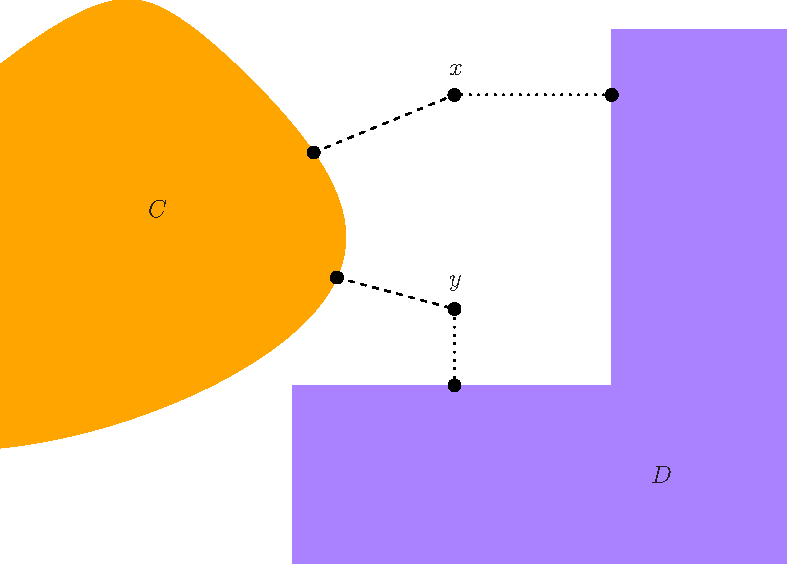
\includegraphics[width=0.65\textwidth]{fig/projection.pdf}
\caption{Illustration of properties of Euclidean projection operators onto 
  convex and nonconvex sets, $C$ and $D$. The projections of $x$ and $y$ onto
  $C$ (visualized via dashed lines) can only grow closer in Euclidean norm,
  whereas their projections onto  $D$ (dotted lines) can spread apart.}    
\label{fig:projection}
\end{figure}

\paragraph{Orthogonal decomposition.}

For a linear subspace $L$, it holds that
\index{projection!orthogonal decomposition}
\begin{equation}
\label{eq:projection_decomposition}
P_L(x) + P_{L^\perp}(x) = x, \quad \text{for all $x$},
\end{equation}
where $L^\perp = \{x : x^\T y = 0, \, \text{for all $y \in L$} \}$ denotes the
orthogonal complement of $L$, which, as it turns out, is itself a linear
subspace. An interesting application of the orthogonal decomposition property
\eqref{eq:projection_decomposition} occurs when $L = \row(A)$ and $L^\perp =
\nul(A)$, the row and null space of a matrix $A$, and this explains the
relationship between the projection maps onto $\row(A)$ and $\nul(A)$ in Example
\parref{xa:matrix_space_projection}. 

The orthogonal decomposition fact \eqref{eq:projection_decomposition} for linear
subspaces is straightforward to verify. From the variational inequality
\eqref{eq:variational_inequality} for projection onto $L$, denoting $z = P_L(x)$,
we first note that this is actually equivalent to a variational \emph{equality}
\begin{equation}
\label{eq:variational_equality}
(x - z)^\T (z - y) = 0, \quad \text{for any $y \in L$}. 
\end{equation}
as $v = z - y$ with $z, y \in L$ implies $v \in L$, and hence $-v \in L$. The 
corresponding variational equality for \smash{$z' = P_{L^\perp}(x)$} is
therefore     
\[
(x - z')^\T (z' - y') = 0, \quad \text{for any $y' \in L^\perp$}.
\]
This is satisfied for $z' = x - z$, as we get $z^\T (x - z - y') = z^\T (x -
z) + z^\T y' = 0 + 0$ for any $y' \in L^\perp$, the first term being zero due to 
\eqref{eq:variational_equality} with $y = 0$, and the second term being zero due
to the fact that $z \in L$ and $y' \in L$. This confirms \smash{$P_{L^\perp}(x) 
  = x - P_L(x)$} and proves \eqref{eq:projection_decomposition}.   

\section{Proximal nonexpansiveness*}
\label{sec:proximal_nonexpansiveness}

We examine firm nonexpansiveness of the proximal mapping. As usual, we take $f$
to be closed and convex, and $\lambda > 0$. Just as we saw for projection maps
onto convex sets, it turns out that $\prox_f$ is \emph{firmly nonexpansive},  
\index{proximal mapping!firm nonexpansiveness}
\begin{equation}
\label{eq:proximal_firm_nonexpansiveness1}
\big( \prox_{\lambda f}(x) - \prox_{\lambda f}(y) \big)^\T (x - y) \geq 
\| \prox_{\lambda f}(x) - \prox_{\lambda f}(y) \|_2^2, \quad \text{for all  
  $x,y$},   
\end{equation}
This is a powerful property, but verifying it is straightforward (in a way, it
is simpler to verify than the corresponding result for projections; recall 
Exercise  \ref{ex:projection_firm_nonexpansiveness}), once we invoke the
appropriate tools: the proximal subgradient characterization, and subgradient 
monotonicity. To see this, without loss of generality, we take $\lambda = 1$,
and abbreviate $z_x = \prox_f(x)$ and $z_y = \prox_f(y)$. Observe that 
\[
(z_x - z_y)^\T (x - y) = (z_x - z_y)^\T \big((x - z_x) - (y - z_y)\big) + 
\|z_x - z_y\|_2^2.   
\]
By the proximal subgradient characterization
\eqref{eq:proximal_subgradient_characterization}, note that $x - z_x \in
\partial f(z_x)$ and $y - z_y \in \partial f(z_y)$; thus by subgradient
monotonicity \eqref{eq:subgradient_monotonicity}, the first term on the
right-hand side above is nonnegative. This proves the firm nonexpansiveness of
$\prox_f$, as desired.   

Again, as in the case of projections (proved in part d of Exercise
\ref{ex:projection_firm_nonexpansiveness}), firm nonexpansiveness
\eqref{eq:proximal_firm_nonexpansiveness1} implies the more evocative  
property   
\begin{equation}
\label{eq:proximal_firm_nonexpansiveness2}
\| \prox_{\lambda f}(x) - \prox_{\lambda f}(y) \|_2^2 + 
\| (I-\prox_{\lambda f})(x) - (I-\prox_{\lambda f})(y) \|_2^2 \leq 
\|x - y\|_2^2, \quad \text{for all $x,y$}, 
\end{equation}
from which we can see that proximal \emph{nonexpansiveness} and \emph{residual
  nonexpansiveness} follow,   
\index{proximal mapping!nonexpansiveness}
\index{proximal mapping!residual nonexpansiveness} 
\begin{align}
\label{eq:proximal_nonexpansiveness}
\|\prox_{\lambda f}(x) - \prox_{\lambda f}(y)\|_2 &\leq \|x-y\|_2, 
\quad \text{for all $x,y$}, \\
\|(I-\prox_{\lambda f})(x) - (I-\prox_{\lambda f})(y)\|_2 &\leq \|x-y\|_2,
 \quad \text{for all $x,y$},
\end{align}
respectively.

\section{Moreau regularization*}
\label{sec:moreau_envelope} 

In this last section, we return to discussing the Moreau envelope $f_\lambda$ of
a closed convex function $f$, as defined in \eqref{eq:moreau_envelope_lambda}.
Repeating its definition here for convenience, for $\lambda > 0$:
\index{Moreau envelope}
\[
f_\lambda(x) = \inf_z \bigg\{ \frac{1}{2\lambda} \|x - z\|_2^2 + f(z)
\bigg\}.
\]
The Moreau envelope $f_\lambda$ can be seen as a smoothed or regularized version
of $f$, and accordingly it is also called \emph{Moreau regularization}. Figure
\ref{fig:moreau_envelope} provides an illustration. More can be said about the 
precise connection between $f_\lambda$ and regularization, and this will be
revisited in the next chapter from the perspective of conjugate functions.      

\begin{figure}[tb]
\centering
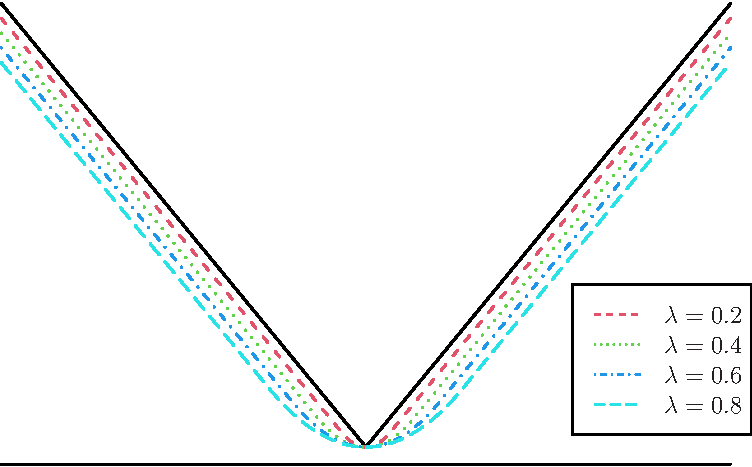
\includegraphics[width=0.625\textwidth]{fig/moreau_envelope.pdf}
\caption{Convex function (solid line) along with its Moreau envelope plotted at
  some values of $\lambda > 0$ (dashed or dotted lines). The Moreau envelope is
  always a differentiable convex minorant to the original function, for any
  $\lambda > 0$.}      
\label{fig:moreau_envelope}
\end{figure}

Several important properties of $f_\lambda$ are apparent. First, the Moreau
envelope $f_ \lambda$ is itself convex (by Property
\parref{par:function_infimum}). Second, $f_\lambda$ has full domain,
$\dom(f_\lambda) = \R^d$, even when the original function $f$ does not. Third, 
$f$ is minorized by its Moreau envelope,
\[
f_\lambda(x) \leq f(x), \quad \text{for all $x$}.
\]
Fourth, the point $z = \prox_{\lambda f}(x)$ achieves the infimum in
\eqref{eq:moreau_envelope_lambda} (see Exercise \ref{ex:moreau_envelope} part
a):  
\begin{equation}
\label{eq:moreau_envelope_prox}
f_\lambda(x) = \frac{1}{2\lambda} \|x - \prox_{\lambda f}(x)\|_2^2 + 
f \big( \prox_{\lambda f}(x) \big).
\end{equation} 
Fifth, the functions $f_\lambda$ and $f$ have the same set of minimizers (see
Exercise \ref{ex:moreau_envelope} part b): 
\begin{equation}
\label{eq:moreau_envelope_argmin}
\argmin_x \, f_\lambda(x) = \argmin_x \, f(x),
\end{equation}
which means that minimization of $f$ and of $f_\lambda$ are equivalent
problems. Sixth, and perhaps most importantly, the Moreau envelope $f_\lambda$
is differentiable, and satisfies  
\index{Moreau envelope!gradient}
\begin{equation}
\label{eq:moreau_envelope_gradient}
\nabla f_\lambda(x) = \frac{1}{\lambda} \big( x - \prox_{\lambda f}(x) \big).  
\end{equation}
This fact is always true regardless of the smoothness of $f$; it is not as
immediately apparent as the above facts, and its proof is outlined in Exercise
\ref{ex:moreau_envelope} parts c and d.  

This latter property, on smoothness of the Moreau envelope, is useful for many
reasons. First, it has important algorithmic implications, as minimization of
$f$ and $f_\lambda$ are equivalent problems \eqref{eq:moreau_envelope_argmin},
and the latter function is always smooth and admits a clean formula
\eqref{eq:moreau_envelope_gradient} for its gradient. Second, it yields a more
rigorous perspective on interpreting the proximal mapping via gradient descent,
as discussed earlier: rearranging \eqref{eq:moreau_envelope_gradient}, we see
that for all $x$ and all $\lambda > 0$,   
\begin{equation}
\label{eq:proximal_gradient_step}
\prox_{\lambda f}(x) = x - \lambda \nabla f_\lambda(x).
\end{equation}
In other words, the proximal map of $\lambda f$ at $x$ is precisely a gradient
step with respect to the Moreau envelope $f_\lambda$ at $x$. Note that
\eqref{eq:proximal_gradient_step} is a more precise version of the earlier 
interpretation \eqref{eq:proximal_gradient_step_approx}: the latter replaces
$\nabla f_\lambda(x)$ by $\nabla f(x)$, which is a reasonable approximation 
for small $\lambda$.    

The third implication of the gradient relation
\eqref{eq:moreau_envelope_gradient} requires a bit more background to
explain. It turns out that the Moreau envelope is a uniquely identifying
transform, in the following sense: if two closed convex functions have matching
Moreau envelopes, then they must be the same function. Further, the relationship
between the proximal map and the gradient of the Moreau envelope
\eqref{eq:moreau_envelope_gradient} transfers the same identifiability property
over to the former (up to an additive constant). We state these results next, to
conclude the chapter.        

\index{Moreau envelope!identification theorem}
\index{proximal mapping!identification theorem}
\begin{Theorem}
\label{thm:moreau_proximal_identification}
For closed convex $f,g : \R^d \to (-\infty, \infty]$ with nonempty domains, the
following properties hold, for any fixed $\lambda > 0$: 
\begin{enumerate}[label=(\roman*)]
\item if $f_\lambda = g_\lambda$, then $f = g$; 
\item if $\prox_{\lambda f} = \prox_{\lambda g}$, then $f = g + c$, for some
  constant $c \in \R$.  
\end{enumerate} 
\end{Theorem}

% Theorem 3.34 and Corollary 3.37 in Rockafellar and Wets (2009)

We call this the \emph{identification theorem} for Moreau envelopes and proximal
mappings; its proof is outlined in Exercise
\ref{ex:moreau_proximal_identification}.  

\SkipTocEntry\section*{Chapter notes}

The notion of a proximal map is attributed to Jean Jacques Moreau, who published  
seminal papers on the topic in the 1960s, including \cite{moreau1962fonctions,
  moreau1963inf, moreau1963proprietes, moreau1965proximite}. Moreau examined the 
ways in which proximal maps generalize projections, and developed (what is now
called) the Moreau envelope. Some authors instead call this Moreau-Yosida
regularization, to recognize earlier related work in functional analysis by
Kosaku Yosida \cite{yosida1948differentiability}. To learn more about proximal
operators and the history behind them, we refer to
\cite{rockafellar2009variational} (Chapters 1.G, 2.D, 3.D), and also to the
monograph \cite{parikh2013proximal}, which gives numerous interesting
interpretations and examples. The connection between the proximal operator and
the resolvent of the subdifferential operator is due to
\cite{rockafellar1976monotone}. For an elegant treatment of this and related
topics from the perspective of monotone operator theory, we refer to
\cite{bauschke2011convex}.

The proximal map of the total variation (TV) seminorm defines a minimization
problem known as \emph{total variation denoising}. This was proposed by
\cite{rudin1992nonlinear}, and led to a large following in research across
applied mathematics, signal processing, and statistics. An important
contribution in statistics that develops this idea further, under the name
\emph{fused lasso}, is \cite{tibshirani2005sparsity}. The taut string algorithm
for TV denoising---that is, for computing the proximal map of the TV
seminorm---was developed by \cite{davies2001local}, building on earlier work by
\cite{mammen1997locally}. A dynamic programming approach for solving the TV
denoising problem was given in \cite{johnson2013dynamic}. The taut string and
dynamic programming algorithms are both linear-time. To be clear, this is all in
reference to the univariate TV denosing problem; for generalizations defined
over multivariate lattices or arbitrary undirected graphs, the computation can
be more challenging. Important algorithmic contributions to more general TV 
denoising settings include \cite{chambolle2009total, chambolle2011first,
  barbero2018modular}, among many others. 

The sorted $\ell_1$ penalty (SLOPE) was proposed by \cite{bogdan2015slope}. 
These same authors presented a fast algorithm for its proximal map by reducing
the problem to isotonic projection, which can be solved in linear-time using the
pool adjacent violators algorithm (PAVA) of \cite{barlow1972statistical}. See
also \cite{deleeuw2010isotonic} for a nice review of various fast algorithms for
isotonic regression and related problems. Projection onto the probability
simplex (and projection onto the $\ell_1$ ball, which is reducible to the
former) can be done in in nearly linear-time with a deterministic algorithm, or
expected linear-time with a randomized algorithm, see \cite{duchi2008efficient, 
  condat2016fast}.   

Insights into the proximal decomposition phenomenon
\eqref{eq:proximal_general_sum}, including fairly general sufficient conditions,
were given in \cite{yu2013decomposing}. This reproduces (and generalizes)
previously known results about proximal decomposition in special cases, such as 
those found in \cite{friedman2007pathwise}, on the elastic net and fused lasso 
penalties. Exercise \ref{ex:proximal_general_sum} is based on
\cite{yu2013decomposing}.     

\clearpage

\begin{xcb}{Exercises}
\begin{enumerate}[label=\thechapter.\arabic*]
\settowidth{\leftmargini}{0.00.\hskip\labelsep}

\item \label{ex:lp_norm_proximal_mapping} 
  We establish the proximal results for the $\ell_1$, $\ell_2$, and $\ell_0$
  norms in Example \ref{xa:proximal_mappings}. 

\begin{enumerate}[label=\alph*.]
\index{l1 norm@$\ell_1$ norm!proximal mapping}
\index{soft-thresholding}
\item Using the subgradient characterization
  \eqref{eq:proximal_subgradient_characterization} and the subgradients
  of the $\ell_1$ norm from Example \parref{xa:l1_norm_subgradients}, prove the
  result in Example \parref{xa:l1_norm_proximal_mapping}.

\item Using the subgradient characterization
  \eqref{eq:proximal_subgradient_characterization} and the subgradients
  of the $\ell_2$ norm from Example \parref{xa:lp_norm_subgradients}, prove the
  result in Example \parref{xa:l2_norm_proximal_mapping}.

\index{l0 norm@$\ell_0$ norm!proximal mapping}
\index{hard-thresholding}
\item Now prove the result in Example \parref{xa:l0_norm_proximal_mapping} on 
  the $\ell_0$ norm, by breaking the argument down into cases (for $|x_i| >
  \lambda$ and $|x_i| \leq \lambda$), and simply arguing directly that the
  minimizer is as claimed in each case.   
\end{enumerate}

\item \label{ex:matrix_norm_proximal_mapping1}
  We establish the proximal results for the trace and Frobenius norms in Example
  \ref{xa:proximal_mappings}. To be entirely clear, for a function $f$ defined
  on $\R^{k \times d}$, its proximal map is  
  \begin{equation}
  \label{eq:proximal_mapping_matrix}
  \prox_{\lambda f}(X) = \argmin_z \bigg\{ \frac{1}{2} \|X -
  Z\|_F^2 + \lambda f(Z) \bigg\}, 
  \end{equation}
  which is consistent with interpreting the space $k \times d$ of matrices as a
  $kd$-dimensional vector space defined by its entries, and applying the usual
  definition \eqref{eq:proximal_mapping_lambda} of the proximal map. The
  subgradient optimality condition for \eqref{eq:proximal_mapping_matrix} says  
  that $Z = \prox_{\lambda f}(X)$ if and only if
  \begin{equation}
  \label{eq:proximal_subgradient_characterization_matrix}
  X - Z \in \lambda \partial f(Z),
  \end{equation}
  which is just the appropriate translation of the subgradient characterization
  \eqref{eq:proximal_subgradient_characterization} to the matrix domain. 

\begin{enumerate}[label=\alph*.]
\index{trace norm!proximal mapping}
\index{matrix soft-thresholding}
\item Using the subgradient characterization 
  \eqref{eq:proximal_subgradient_characterization_matrix} along with the
  subgradients of the trace norm from Example
  \parref{xa:trace_norm_subgradients}, prove the result in Example
  \parref{xa:trace_norm_proximal_mapping}. 

\index{Frobenius norm!proximal mapping}
\item Using the subgradient characterization 
  \eqref{eq:proximal_subgradient_characterization_matrix}, where the
  subgradients of the Frobenius norm can derived analogously to those for the
  $\ell_2$ norm as in Example \parref{xa:lp_norm_subgradients}, prove the result
  in Example \parref{xa:frobenius_norm_proximal_mapping}.  
\end{enumerate}

\item \label{ex:matrix_norm_proximal_mapping2}
  Now we derive proximal mappings for a class of functions on $\R^{k \times d}$,
  of the form 
  \begin{equation}
  \label{eq:singular_function}
  f(X) = g(\sigma(X)), 
  \end{equation}
  for a function $g : \R^d \to \R$, where we write $\sigma(X) = (\sigma_1(X), \dots,
  \sigma_k(X)) \in \R^k$ for the vector of singular values of $X$. An important
  example here is the \emph{Schatten $p$-norm}, defined for $p \geq 1$ as
  \index{Schatten norm}
  \begin{equation}
  \label{eq:schatten_norm}
  \|X\|_p = \|\sigma(X)\|_p,
  \end{equation}
  with $\|\cdot\|_p$ on the right-hand side denoting the usual $\ell_p$ norm on
  vectors. Note that in terms of Shatten norms (that is, the left-hand side in
  all equalities below represents a Schatten norm): 
  \begin{itemize}
  \item $\|\cdot\|_1 = \|\cdot\|_{\tr}$, the trace norm;
  \item $\|\cdot\|_2 = \|\cdot\|_F$, the Frobenius norm; and
  \item $\|\cdot\|_\infty = \|\cdot\|_{\op}$, the operator norm.  
  \end{itemize}
  An important fact about functions $f$ of the form
  \eqref{eq:singular_function}: they are \emph{unitarily invariant}, meaning 
  $f(UXV) = f(X)$ for any orthogonal matrices $U,V$ (because left- or
  right-muliplication by orthogonal matrices does not change the singular
  values).    
  
\begin{enumerate}[label=\alph*.]
\item For $X = U \Sigma V^\T$ denoting the SVD of $X$, and $\sigma = \sigma(X)$
  is the diagonal of $\Sigma$, prove   
  \[
  \prox_{\lambda f}(X) = U \diag(\prox_g(\sigma)) V^\T,
  \]
  where we use $A = \diag(a)$ to construct a diagonal matrix from a vector $a$.    

\item Using the Schatten $p$-norm connections listed above, check that the
  result from part a reproduces the results for the trace and Frobenius norms, in
  Examples \parref{xa:trace_norm_proximal_mapping} and 
  \parref{xa:frobenius_norm_proximal_mapping}.  
\index{Schatten norm!proximal mapping}
  
\item Now use the result from part a to derive the proximal map of the matrix
  rank function, from Example \parref{xa:rank_proximal_mapping}. 
\end{enumerate}

\item For \smash{$f(x) = \inf_{z \in C} \|x - z\|_2 = \|x - P_C(x)\|_2$},
  where $C$ is a closed convex set, prove that   
  \[
  \prox_{\lambda f}(x) = 
  \begin{cases}
  \displaystyle
  x - \lambda \frac{x - P_C(x)}{\|x - P_C(x)\|_2} & 
  \text{if $\|x - P_C(x)\|_2 > \lambda$} \\ 
  P_C(x) & \text{if $\|x - P_C(x)\|_2 \leq \lambda$}.
  \end{cases}
  \]
  Hint: recall that $f$ is differentiable at each $x \notin C$, with gradient
  given in \eqref{eq:set_distance_subgradients}.    

\item Prove the proximal quadratic sum rule in Property
  \parref{par:proximal_quadratic_sum}.  

\item \label{ex:generalized_enet_proximal_mapping}
  Prove the proximal decomposition fact 
  \eqref{eq:generalized_enet_proximal_mapping} for positively homogeneous 
  $f$. Hint: show that positive homogeneity implies that $\prox_{tf}(tx) = t
  \prox_f(x)$, for any $t > 0$ and any $x$; use this together with the quadratic
  sum rule from Property \parref{par:proximal_quadratic_sum} to prove the
  desired result.  

\item \label{ex:proximal_general_sum}
  In this exercise, we will establish a sufficient condition for the
  proximal decomposition given in \eqref{eq:proximal_general_sum}, following the
  development of Theorem 1 and Proposition 2 in \cite{yu2013decomposing}. Let  
  $f,g$ be closed and convex.   

\begin{enumerate}[label=\alph*.]
\item First show that, for any $x$, the point $\prox_f(\prox_g(x))$ satisfies  
  \[
  0 \in \prox_f(\prox_g(x)) - x + \partial g(\prox_g(x)) + 
  \partial f \big( \prox_f(\prox_g(x)) \big).
  \]
  Hint: use the proximal subgradient characterization
  \eqref{eq:proximal_subgradient_characterization} for $\prox_f(\prox_g(x))$, 
  as well as for $\prox_g(x)$, and add these two expressions together. 

\item Assume that 
  \begin{equation}
  \label{eq:proximal_decomposition_condition1}
  \partial g(x) \subseteq \partial g(\prox_f(x)), \quad \text{for all $x$}. 
  \end{equation}
  Show that, for any $x$, the point $\prox_f(\prox_g(x))$ must then satisfy   
  \[
  0 \in \prox_f(\prox_g(x)) - x + \partial g \big( \prox_f(\prox_g(x)) \big) +  
  \partial f \big( \prox_f(\prox_g(x)) \big).
  \]
  Hint: use part a. Conclude using the subgradient characterization for
  $\prox_{f+g}(x)$ and single-valuedness of the proximal map that
  $\prox_{f+g}(x) = \prox_f(\prox_g(x))$, and as $x$ was arbitrary,
  $\prox_{f+g} =  \prox_f \circ \prox_g$.   

\item Let \smash{$g = \sum_{i=1}^k g_i$}, with each $g_i$ closed and convex, 
  and \smash{$\cap_{i=1}^k \relint(\dom(g_i)) \not= \emptyset$}. Prove that
  \eqref{eq:proximal_decomposition_condition1} is implied by
  \begin{equation}
  \label{eq:proximal_decomposition_condition2}
  \partial g_i(x) \subseteq \partial g_i(\prox_f(x)), \quad \text{for all $x$, 
    and $i=1,\dots,k$},  
  \end{equation}
  and thus the latter is a sufficient condition for $\prox_{f+g} =  \prox_f \circ
  \prox_g$. 
\end{enumerate}

\item \label{ex:generalized_tv_proximal_mapping}
  Now we follow the development of Corollary 4 in \cite{yu2013decomposing}. Let
  $g$ be a polyhedral function, 
  \[
  g(x) = \max_{i=1,\dots,k} \, a_i^\T x.
  \]
  
\begin{enumerate}[label=\alph*.]
\item Show that the sufficient condition in
  \eqref{eq:proximal_decomposition_condition2}, from Exercise
  \ref{ex:proximal_general_sum} part c, is equivalent to  
  \[
  \prox_g(K_i) \subseteq K_i, \quad i=1,\dots,k,
  \]
  where each $K_i = \{x : a_i^\T x = g(x)\}$ is a polyhedral cone. Hint: use the
  subgradient rule for a pointwise maximum from Property
  \parref{par:subgradient_supremum}.   

\item Let $f$ be permutation invariant, which means that $f(x) = f(x_\pi)$, for
  all $x$ and permutations $\pi$ (where we denote \smash{$x_\pi = (x_{\pi_1},
    \dots, x_{\pi_d})$} for $\pi=(\pi_1,\dots,\pi_d)$). Show that $\prox_f$ is
  then order-preserving,  
 \[
 x_i \geq x_j \implies [\prox_f(x)]_i \geq [\prox_f(x)]_j, \quad \text{for all
   $x \in \R^d$ and $i,j$}.
 \]

\item Let \smash{$\|x\|_{\TV} = \sum_{(i,j) \in E} |x_i - x_j|$} be a
  generalized TV seminorm, defined with respect to an edge set $E$ (notice that  
  this generalizes \eqref{eq:tv}, which corresponds to $E = \{(i, i+1) : i =
  1,\dots,d-1\}$. Prove that \eqref{eq:generalized_tv_proximal_mapping} holds
  for any permutation invariant $f$ and any edge set $E$. Hint: check that the
  condition in part a holds, for the appropriate instantiation of cones $K_i$,
  $i=1,\dots,k$; and for this, use the order-preserving property from part b.   
\index{total variation (TV) penalty!proximal mapping}
\end{enumerate}

\item \label{ex:proximal_linear}
  We examine linear composition rules for proximal mappings. 

\begin{enumerate}[label=\alph*.]
\item Prove the rule in Property \parref{par:proximal_linear} for orthogonal $A$
  (that is, $A^\T A = A A^\T = I$).   

\item Prove that more generally, if $A$ has orthonormal rows (and it need not be 
  square), and $b \in \R^d$ is arbitrary, then $F(x) = f(Ax + b)$ has proximal
  mapping 
  \[
  \prox_F(x)  = x - A^\T \big(Ax + b - \prox_f(Ax + b) \big).
  \]
\end{enumerate}
  
\index{proximal mapping!fixed-point equation}
\item \label{ex:proximal_optimality_fg}
  In this exercise, we prove that the fixed-point equation 
  \eqref{eq:proximal_optimality_fg} is necessary and sufficient for minimizing
  $F = f+g$, where $f,g$ are closed and convex and $f$ is differentiable. Let
  $\lambda > 0$ be arbitrary.

\begin{enumerate}[label=\alph*.]
\item Assuming $\interior(\dom(f)) \cap \relint(\dom(g)) \not= \emptyset$, show
  that $x$ minimizes $F$ if and only if   
  \[
  x - \lambda \nabla f(x) \in x + \lambda \partial g(x).
  \]
  
\item Show that the above display is equivalent to
  \eqref{eq:proximal_optimality_fg} using the resolvent characterization     
  $\prox_{\lambda g} = (I + \lambda \partial g)^{-1}$, and the fact that this
  inverse is single-valued. 
\end{enumerate}

\index{projection!onto $\ell_1$ ball}
\index{probability simplex!projection}
\item \label{ex:l1_projection}
  Consider the projection problems for the probability simplex and the unit
  $\ell_1$ ball, 
  \begin{align}
  \label{eq:simplex_projection}
  &\minimize_z \quad \|x - z\|_2^2 \quad \st \quad \one^\T z = 1, 
    \; z \geq 0, \\ 
  \label{eq:l1_projection}
  &\minimize_z \quad \|x - z\|_2^2 \quad \st \quad \|z\|_1 \leq 1,
  \end{align}
  respectively. 

\begin{enumerate}[label=\alph*.]
\item Show that if $z$ is a solution in \eqref{eq:l1_projection}, then
  $\sign(z_i) = \sign(x_i)$, $i=1,\dots,d$.    

\item Use part a to argue that we can reduce any $\ell_1$ projection to a
  simplex projection. That is, in order to solve \eqref{eq:l1_projection}, we
  can first solve a problem of the form \eqref{eq:simplex_projection}, and then 
  we can postprocess the solution to obtain a solution to the original problem.     
\end{enumerate}  

\index{projection!firm nonexpansiveness}
\item \label{ex:projection_firm_nonexpansiveness}
  This exercise investigates firm nonexpansiveness
  \eqref{eq:projection_firm_nonexpansiveness1} of the projection operator $P_C$
  onto a convex set $C$. For any $x,y$, let us abbreviate $p_x = P_C(x)$ and
  $p_y = P_C(y)$. From the variational inequality
  \eqref{eq:variational_inequality}, note that     
  \begin{align*}
  (x - p_x)^\T (p_x - y) \geq 0, \\
  (y - p_y)^\T (p_y - x) \geq 0.
  \end{align*}

\begin{enumerate}[label=\alph*.]
\item Use the above pair of inequalities to prove that 
  \[
  \big( x - p_x - (y - p_y) \big)^\T (p_x - p_y) \geq 0, \quad \text{for all
    $x,y$}. 
  \]
  Hint: expand $p_x - y = p_x - p_y + p_y - y$ in the first inequality, $p_y - x
  = p_y - p_x + p_x - x$ in the second inequality, then subtract the two and
  simplify.   
  
\item Show that the condition from part a is equivalent to firm nonexpansiveness 
  \eqref{eq:projection_firm_nonexpansiveness1}, and show that it also equivalent
  to   
  \[
  (r_x - r_y)^\T (x - y) \geq \|r_x - r_y\|_2^2, \quad \text{for all $x,y$},
  \]
  where we abbreviate $r_x = x - P_C(x)$ and $r_y = x - P_C(y)$.

\item Show using the Cauchy-Schwarz inequality that
  \eqref{eq:projection_firm_nonexpansiveness1} implies
  \eqref{eq:projection_nonexpansiveness}. Show similarly using part b and the
  Cauchy-Schwarz inequality that \eqref{eq:projection_firm_nonexpansiveness1}
  implies \eqref{eq:projection_residual_nonexpansiveness}.

\item Show finally that firm nonexpansiveness implies 
  \[
  \|p_x - p_y\|_2^2 + \|r_x - r_y\|_2^2 \leq \|x - y\|_2^2, \quad \text{for all
    $x,y$},
  \]
  which gives another way of seeing that
  \eqref{eq:projection_firm_nonexpansiveness1} leads to both
  \eqref{eq:projection_nonexpansiveness} and
  \eqref{eq:projection_residual_nonexpansiveness}. 
\end{enumerate}

\index{proximal mapping!contractiveness}
\index{proximal mapping!fixed-point equation}
\item In this exercise, we study a \emph{contractive} property of proximal
  operators (and projections): for closed convex $f$ and $\lambda > 0$, show
  that if $f(x^\star) = f^\star = \inf_x f(x)$, then   
  \[
  \| \prox_{\lambda f}(x) - x^\star\|_2 < \|x - x^\star\|_2, \quad \text{for
    all $x$ with $f(x) > f^\star$}.
  \]
  Note the strict inequality. In the special case of $f = I_C$, the
  characteristic function of a closed convex set $C$, this reduces to 
  \[
  \| P_C(x) - y\|_2 < \|x - y\|_2, \quad \text{for all $x \notin C$ and $y \in
    C$}.    
  \]
  Hint: recall the implication \eqref{eq:proximal_firm_nonexpansiveness2} from
  firm nonexpansiveness, and the proximal fixed-point characterization of 
  minimizers in \eqref{eq:proximal_optimality}.  

\item \label{ex:moreau_envelope}
  We examine key facts about the Moreau envelope $f_\lambda$ of a closed convex
  function $f$, for $\lambda > 0$. 

\begin{enumerate}[label=\alph*.]
\item Prove the property given in \eqref{eq:moreau_envelope_prox}. Hint: apply
  the subgradient optimality condition to the optimization problem that defines 
  $f_\lambda(x)$.     
 
\item Show that $f$ and $f_\lambda$ have the same minimizers
  \eqref{eq:moreau_envelope_argmin}. Hint: use \eqref{eq:moreau_envelope_prox}
  and the proximal optimality condition \eqref{eq:proximal_optimality}. 

\item Show that if $f_\lambda$ were differentiable, then its gradient must be as
  in \eqref{eq:moreau_envelope_gradient}, by using the subgradient rule for a
  partial infimum in Property \parref{par:subgradient_infimum}.   

\index{Moreau envelope!gradient}
\item Now prove that $f_\lambda$ is differentiable with gradient as given in
  \eqref{eq:moreau_envelope_gradient}. Hint: abbreviating $f_x = f_\lambda(x)$
  and $z_x = \prox_{\lambda f}(x)$, simply verify the definition of
  differentiability directly: 
  \[
  \lim_{y \to x} \frac{f_y - f_x - (y - x)^\T (x - z_x) / \lambda}{\|y-x\|_2^2} 
  = 0.
  \]
  To check this, use \eqref{eq:moreau_envelope_prox} and direct algebra to argue 
  that $f_y - f_x \geq (y - x)^\T (x - z_x) / \lambda$; by swapping the roles of
  $x$ and $y$, argue that also $f_y - f_x \leq (y - x)^\T (y - z_y) / \lambda$. 
  These two inequalities can be used in combination to verify the
  differentiability condition.     
\end{enumerate}

\item Let $f(x) = |x|$. Prove that its Moreau envelope $f_\lambda$ is the 
  \emph{Huber function} (which is commonly used as a loss in robust statistics,
  being smooth and having linear growth away from zero): 
  \index{Huber function}
  \[
  f_\lambda(x) = 
  \begin{cases}
  x^2/ (2\lambda) & \text{if $|x| \leq \lambda$} \\
  |x| - \lambda/2 & \text{if $|x| > \lambda$}.
  \end{cases}
  \]
  This is in fact the Moreau envelope that is visualized in Figure
  \ref{fig:moreau_envelope}.  

\index{Moreau envelope!identification theorem}
\index{proximal mapping!identification theorem}
\item \label{ex:moreau_proximal_identification}
  In this exercise, we prove the identification theorem, Theorem
  \ref{thm:moreau_proximal_identification}, for Moreau envelopes and proximal
  maps. Following the development of Theorem 3.34 in
  \cite{rockafellar2009variational}, it helps to introduce the general concept 
  of an \emph{infimal convolution} of functions $f,g$: 
  \index{infimal convolution}
  \[
  (f \infconv g)(x) = \inf_z \Big\{ f(z) + g(x-z) \Big\}.
  \]
  In this notation, observe that \smash{$f_\lambda = f \infconv \|\cdot\|_2^2 / 
    (2\lambda)$}, that is, the Moreau envelope is the infimal convolution of $f$
  and the map $x \mapsto \|x\|_2^2 /  (2\lambda)$. Below, let $f,g$ be closed
  and convex.   

\begin{enumerate}[label=\alph*.]
\item Assume that $f \infconv h = g \infconv h$ for a closed, convex, and
  coercive function $h$. Prove that for any value of $\lambda > 0$,  
  \[
  \inf_x \Big\{ f_\lambda(x) - v^\T x \Big\} = \inf_x \Big\{ g_\lambda(x) - v^\T
  x \Big\}, \quad \text{for all $v$}.
  \]
  Hint: first observe that $f_\lambda \infconv h = g_\lambda \infconv h$ by the
  commutative property of infimal convolutions. Then use basic algebra to
  decompose \smash{$\inf_x \, \{ f_\lambda \infconv h(x) - v^\T x \}$} into two 
  terms, one depending only on $f_\lambda$, and the other only on $h$. Compare
  this to the expression we get when $f$ is replaced by $g$. 

\item Now under the same assumption $f \infconv h = g \infconv h$, show that $f
  = g$. Hint: if $f \not= g$ then for some $x$ we will have (without a loss of
  generality) $f(x) > g(x)$, and thus $f_\lambda(x) > g_\lambda(x)$ for small 
  enough $\lambda > 0$. Show that for $v = \nabla f_\lambda(x)$, we get   
  \[
  \inf_y \Big\{ f_\lambda(y) - v^\T y \Big\} = 
  f_\lambda(x) - v^\T x > g_\lambda(x) - v^\T x \geq 
  \inf_y \Big\{ g_\lambda(y) - v^\T y \Big\},
  \]
  which would violate the result from part a.

\item Fix $\lambda > 0$. Apply the result from part b to $h(x) =
  \|x\|_2^2/(2\lambda)$, in order to prove part (i) in Theorem
  \ref{thm:moreau_proximal_identification}. Use the gradient relation
  \eqref{eq:moreau_envelope_gradient} to prove part (ii) in the theorem.  
\end{enumerate}

\index{scaled proximal mapping}
\item \label{ex:scaled_proximal_mapping}
  We explore a generalization of the proximal map known as the \emph{scaled 
    proximal map}. We fix a positive definite matrix $H \succ 0$, and then
  define the scaled proximal mapping with respect to $H$, acting on a given
  function $f$, by   
  \begin{equation}
  \label{eq:scaled_proximal_mapping}
  \prox_f^H(x) = \argmin_z \bigg\{ \frac{1}{2} \|x - z\|_H^2 + f(z) \bigg\}, 
  \end{equation}
  where $\|\cdot\|_H$ denotes the scaled Euclidean norm, defined by $\|x\|_H^2 = 
  x^\T H x$. The parts of this exercise that follow walk through several nice
  properties of the scaled proximal mapping \eqref{eq:scaled_proximal_mapping},
  generalizing those of the (unscaled) proximal mapping
  \eqref{eq:proximal_mapping_lambda}. Note that the former is a special case of 
  the latter with $H = (1/\lambda) I$, with $I$ denoting the identity
  matrix. Below $f$ is assumed to be closed and convex.  

\begin{enumerate}[label=\alph*.]
\item \emph{Existence and uniqueness.} Prove that the minimizer in
  \eqref{eq:scaled_proximal_mapping} exists and is unique.

\item \emph{Subgradient characterization.} Prove that \smash{$z = \prox_f^H(x)$}
  if and only if $H(x - z) \in \partial f(z)$. 

\item \emph{Steepest descent interpretation.} Argue (using heuristic arguments)
  that 
  \[
  \prox_f^H(x) \approx x - H^{-1} \nabla f(x),
  \] 
  which we can interpret as performing a steepest descent step starting at $x$,
  which respect to the scaled norm $\|\cdot\|_H$. 

\item \emph{Resolvent characterization.} Prove that \smash{$\prox_f^H = (H +
    \partial f)^{-1} H$}, where the inverse here is interpreted as
  single-valued.   

\item \emph{Fixed-point equation.} Prove that $x$ minimizes $f$ if and only if
  \smash{$x = \prox_f^H(x)$}; furthermore, $x$ minimizes $F = f+g$ for closed
  convex $f,g$, with $f$ differentiable, if and only if    
  \[
  x = \prox_g^H \big( x - H^{-1} \nabla f(x) \big).
  \]

\item \emph{Firm nonexpansiveness.} Prove that \smash{$\prox_f^H$} is firmly
  nonexpansive in the $\|\cdot\|_H$ norm, 
  \[
  \big( \prox_f^H(x) - \prox_f^H(y) \big)^\T (x - y) \geq 
  \| \prox_f^H(x) - \prox_f^H(y) \|_H^2, \quad \text{for all $x,y$}.   
  \]
  Show that this in turn implies that it is both nonexpansive and residual
  nonexpansive, again in the $\|\cdot\|_H$ norm.
\end{enumerate}
\end{enumerate}
\end{xcb}